\chapter{Estudo de caso (QIE)}
Neste capítulo será descrita a utilização do processo de alinhamento através de uma aplicação real chamada QIE. O QIE foi escolhido como um bom cenário, pois se trata de um projeto que pretende cruzar informações sobre a comunidade brasileira de informática na educação.

Para validar a eficácia da solução, foi solicitado a membros da comunidade que sugerissem perguntas de seu interesse. Como resultado foi levantado um conjunto contendo mais de 30 questões (ver Tabela \ref{tab:questions}).

\begin{table}[!ht]
\centering
\caption{Perguntas sugeridas pela comunidade}
\label{tab:questions}
\begin{tabular}{|l|l|}
\hline
ID  & Questões                                                                          \\ \hline
Q01 & Quantos pesquisadores?                                                            \\ \hline
Q02 & Quais pesquisadores?                                                              \\ \hline
Q03 & Onde estão? (Estado)                                                              \\ \hline
Q04 & Onde estão? (Universidade)                                                        \\ \hline
Q05 & Quais são Doutores?                                                               \\ \hline
Q06 & Quantos são Doutores?                                                             \\ \hline
Q07 & Quem possui marca?                                                                \\ \hline
Q08 & Onde fizemos os nossos doutorados?                                                \\ \hline
Q09 & Onde fizemos os nossos pós-doutorados?                                            \\ \hline
Q10 & Quantas publicações o autor “z” tem no evento “x”?                                \\ \hline
Q11 & Quantos trabalhos foram publicados no evento “x”?                                 \\ \hline
Q12 & Quantos autores publicaram no evento “x”?                                         \\ \hline
Q13 & Quantos artigos foram publicados no periódico “y”?                                \\ \hline
Q14 & Lista de Doutores + Email (RBIE)                                                  \\ \hline
Q15 & Lista de Autores + Competência + Email                                            \\ \hline
Q16 & Lista de Artigos publicados na RBIE - Geral                                       \\ \hline
Q17 & Quantos são bolsistas e qual o nível? (DT/PQ)                                     \\ \hline
Q18 & Quais são as principais competências da comunidade de IE?                         \\ \hline
Q19 & Quais conceitos são explorados?                                                   \\ \hline
Q20 & Quais os temas são mais pesquisados em IE?                                        \\ \hline
Q21 & Quais pesquisadores colaboram entre si?                                           \\ \hline
Q22 & Quais instituições colaboram entre si?                                            \\ \hline
Q23 & Quais são os trabalhos relacionados?                                              \\ \hline
Q24 & Como os conceitos explorados evoluem ao longo do tempo?                           \\ \hline
Q25 & Mapa de tendências de pesquisa em uma linha do tempo.                             \\ \hline
Q26 & O quão um pesquisador X está publicando no SBIE, WIE e RBIE ao longo do tempo?    \\ \hline
Q27 & Lista de bolsistas de produtividade                                               \\ \hline
Q28 & Quais as instituições?                                                            \\ \hline
Q29 & Quais autores publicaram na conferência "X"?                                      \\ \hline
Q30 & Quantos pesquisadores de IE estão em PPGs de CC?                                  \\ \hline
Q31 & Quem são os maiores especialistas em recursos digitais e objetos de aprendizagem? \\ \hline
\end{tabular}
\end{table}

Para responder tais questões é necessário cruzar informações dos pesquisadores e suas respectivas publicações de diferentes bases, sendo elas a Revista Brasileira de Informática na Educação (RBIE), Workshop de informática na Escola (WIE), Simpósio Brasileiro de Informática na Educação (SBIE) e currículum Lattes. Vale a pena ressaltar que os datasets foram disponibilizados como arquivos XML, sendo necessário transformá-los para RDF.

Para modelar os dados, foram utilizadas duas ontologias a dac e a lattes. A primeira tem o objetivo de modelar o domínio de publicação (ver Figura \ref{fig:dac}). A segunda foi construída para modelar o domínio do lattes (ver Figura \ref{fig:lattes}).

\begin{figure}[!ht]
	\centering
	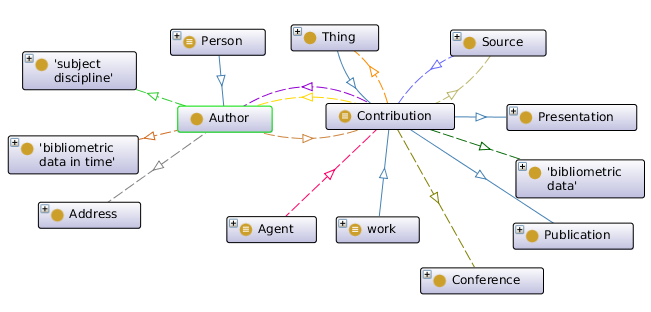
\includegraphics[width=0.9\textwidth]{./imagens/dac-mainview.png}
    \caption{Taxonomia da ontologia dac}
	\label{fig:dac}
\end{figure}

\begin{figure}[!ht]
	\centering
	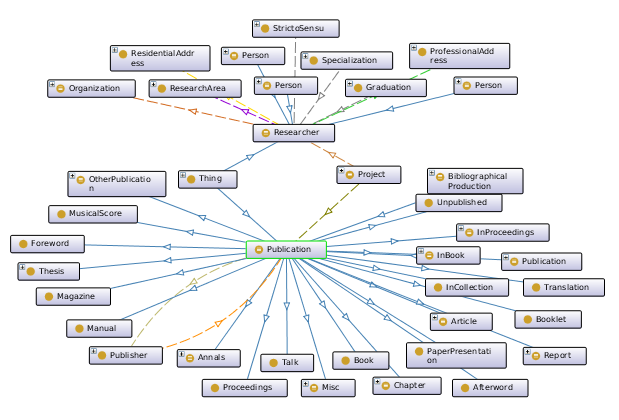
\includegraphics[width=0.9\textwidth]{./imagens/lattes-mainview.png}
    \caption{Taxonomia da ontologia lattes}
	\label{fig:lattes}
\end{figure}

Para converter os dados para RDF foi utilizada a ferramenta OpenRefine com a extensão para suportar RDF. Após a transformação dos dados, as ontologias e os dados são persistidos no Virtuoso (ver Figura \ref{fig:datasets}), que é uma ferramenta para armazenamento de triplas.

\begin{figure}[!ht]
	\centering
	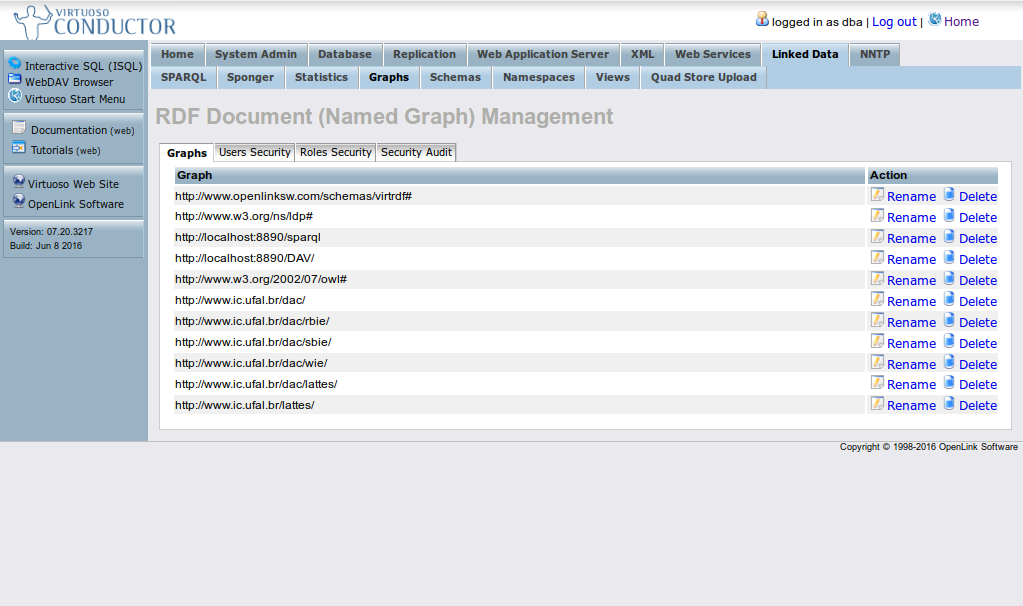
\includegraphics[width=0.9\textwidth]{./imagens/datasets.png}
    \caption{Datasets armazenados na triple store}
	\label{fig:datasets}
\end{figure}

Após a persistência dos dados, o processo de alinhamento foi executado. Vale ressaltar que os datasets também foram alinhados com eles mesmos com o objetivo de descobrir recursos duplicados, visto que um autor pode publicar vários artigos em um mesmo evento. Os alinhamento gerados foram persistidos em novos datasets (ver Figura \ref{fig:datasets_alingments}).

\begin{figure}[!ht]
	\centering
	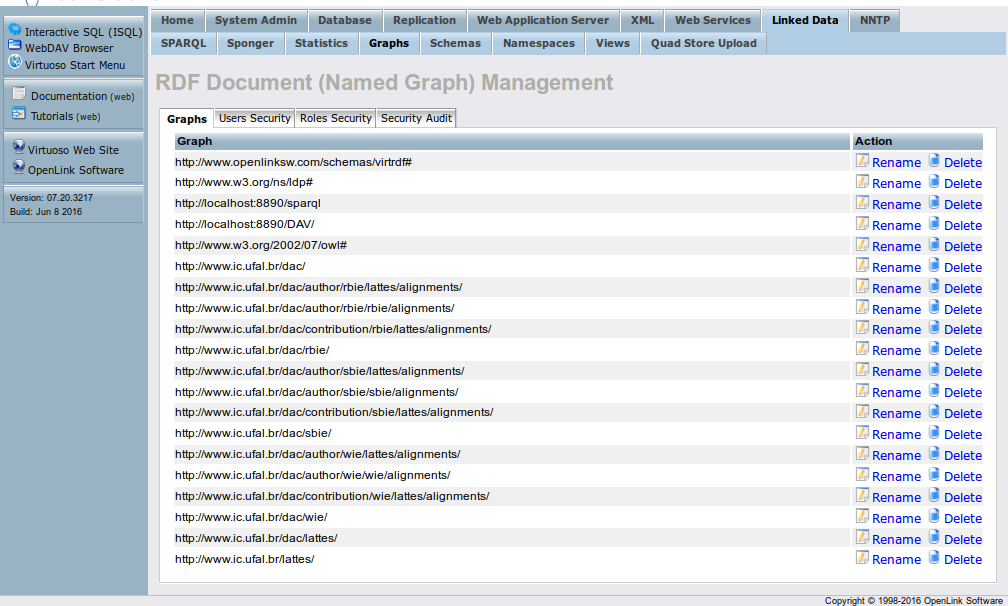
\includegraphics[width=0.9\textwidth]{./imagens/datasets-alinhamento.png}
    \caption{Datasets armazenados na triple store}
	\label{fig:datasets_alingments}
\end{figure}

Após a realização do alinhamento por parte da ferramenta, foi realizado um levantamento. A partir do levantamento foi possível gerar algumas estatísticas sobre esses datasets, sendo eles a quantidade de recursos não repetidos nas bases, total de recursos alinhados com o perfil Lattes, bem como precision, recall e f-measure [citação] para analisar a confiabilidade dos alinhamentos (ver Tabela \ref{tab:case_study}).

\begin{landscape}
\begin{table}[!ht]
\centering
\caption{ Resultado dos alinhamentos com relação aos dados do Lattes}
\label{tab:case_study}
\begin{tabular}{|c|c|c|c|c|c|c|c|}
\hline
Dataset & Alinhamentos & Recursos Alinhados & Iniciais & Finais & Perfis com Lattes (TOTAL) & Perfis com Lattes (Finais) & P | R | F \\ \hline
RBIE & 1276 & 1029 & 1118 & 806 & 92.03\% (1029) & 89.06\% (717) & 0.97 | 1 | 0.98 \\ \hline
SBIE & 1742 & 141 & 1687 & 1032 & 71.54\% (1207) & 70.16\% (792) & 0.94 | 1 | 0.97 \\ \hline
WIE & 1637 & 1405 & 1952 & 1098 & 75.20\% (1468) & 67.48\% (741) & 0.84 | 1 | 0.91 \\ \hline
\end{tabular}
\end{table}
\end{landscape}